\documentclass[twocolumn]{article}
\pdfoutput=1

% Roman numbers for sections
\renewcommand{\thesection}{\Roman{section}} 
\renewcommand{\thesubsection}{\thesection.\Roman{subsection}}

\usepackage{arxiv}

\usepackage[utf8]{inputenc} % allow utf-8 input
\usepackage[T1]{fontenc}    % use 8-bit T1 fonts
\usepackage{hyperref}       % hyperlinks
\usepackage{url}            % simple URL typesetting
\usepackage{booktabs}       % professional-quality tables
\usepackage{amsmath}
\usepackage{enumitem}
\setlist[itemize]{align=parleft,left=0pt..1em}
\setlist[enumerate]{align=parleft,left=0pt..1em}
\usepackage{amsfonts}       % blackboard math symbols
\usepackage{nicefrac}       % compact symbols for 1/2, etc.
\usepackage{microtype}      % microtypography
\usepackage{lipsum}		% Can be removed after putting your text content
\usepackage{graphicx}
\usepackage{natbib}
\usepackage{doi}
\usepackage{listings,xcolor}

\lstdefinestyle{lua}{
  language=[5.3]Lua,
  basicstyle=\ttfamily,
  keywordstyle=\color{magenta},
  stringstyle=\color{blue},
  commentstyle=\color{black!50}
}

\title{Multidarkroom}

%\date{September 9, 1985}	% Here you can change the date presented in the paper title
%\date{} 					% Or removing it

\author{
    Denis Roio \\
	Dyne.org foundation \\
	Amsterdam, 1013AK \\
	\texttt{J@Dyne.org} \\
    \And
	Alberto Ibrisevic \\
	Laboratory of Cryptography\\
	Trento University (stage)\\
	\texttt{bettowski@dyne.org} \\
    \And
    Andrea D'Intino \\
    Dyne.org foundation \\
    Amsterdam, 1013AK \\
    \texttt{Andrea@Dyne.org} \\
}

% Uncomment to remove the date
%\date{}

% Uncomment to override  the `A preprint' in the header
\renewcommand{\headeright}{Dyne.org}
\renewcommand{\undertitle}{Zero Knowledge Multi Party Signatures with
  Application to Distributed Ledgers}
\renewcommand{\shorttitle}{\textit{Multidarkroom}}

\hypersetup{
  pdftitle={Multidarkroom - Zero-knowledge proof secured BLS multi-signatures},
  pdfsubject={cs.CR},
  pdfauthor={Denis Roio, Alberto Ibrisevic, Andrea D'Intino},
  pdfkeywords={Cryptography, signatures, zero-knowledge, multi-party, BLS, Coconut},
}

\begin{document}

\twocolumn[
  \begin{@twocolumnfalse}

\maketitle

\begin{abstract}
  Multidarkroom is a novel signature scheme supporting unlinkable
  signatures by multiple parties authenticated by means of a
  zero-knowledge credential scheme. Multidarkroom integrates with
  blockchains to ensure condidentiality, authenticity and availability
  even when credential issuing authorities are offline. We implement
  and evaluate a Multidarkroom smart contract for Zenroom and present
  an application related to multiple anonymous signatures by
  authenticated parties. Multidarkroom uses short and computationally
  efficient signatures and credentials whose verification takes the
  longest time to compute.
\end{abstract}

\vspace{2cm}

 \end{@twocolumnfalse}
]



\section{Introduction}

Multi-party computation [] applied to the signing process [] allows
the issuance of signatures without requiring any of the participating
parties to disclose secret signing keys to each other, nor requires
the presence of a trusted third-party to receive them and compose the
signatures. However, established schemes have shortcomings. Some do
not provide the necessary efficiency, re-randomization, or blind
issuance properties necessary to implement the privacy preserving
features necessary for the application to trustless distributed
systems. Other schemes are prone to rogue-key attacks \citep{ietf-bls}
in the absence of authentication methods to grant that signatures are
produced by legitimate key holders.

The lack of efficient and privacy-preserving signature schemes impacts
distributed ledger platforms that support 'smart contracts' as well
distributed computing architectures where trust is not shared among
participants, but granted by one or more authorities through
credential issuance for the generation of non-interactive and
unlinkable proofs.

Multidarkroom uses short and computationally efficient signatures
composed of exactly two group elements that are linked to each
other. The size of the signature remains constant regardless of the
number of parties that are signing, while the credential size grows
linearly. Furthermure, after a one-time setup phase where the users
collect and aggregate a threshold number of verification keys from the
autorities, the attribute showing and verification O(1) in terms of
both cryptographic computations and communication of cryptographic
material, irrespective of the number of authorities.

Our evaluationof the Multiparty primities shows very promising
results. Verifiction takes about 10ms,  while signing a document is
about 3 times faster. 

\textbf{Contributions:} This paper makes three key contributions:

\begin{itemize}

\item We describe the signature scheme underlying Multidarkroom,
  including how key generation, signing and verification operate
  (Section \ref{sec:signature}). The scheme is an application of the
  BLS signature scheme \citep{asiacrypt-bls} fitted with features to
  grant the unlinkability of signatures and to secure it against
  rogue-key attacks.

\item We describe the credential scheme underlying Multidarkroom,
  including how key generation, issuance, aggregation and verification
  of credentials operate (Section \ref{sec:credential}). The scheme is
  an application of the Coconut credential scheme \citep{coconut-2018}
  that is general purpose and can be scaled to a fully distributed
  threshold issuance that is re-randomizable.

\item We implement a Zencode scenario of Multidarkroom to be executed
  on and off-chain by the Zenroom VM, complete with functions for
  public credential issuance, signature session creation and
  multi-party non-interactive signing (Section
  \ref{sec:implementation}). We evaluate the performance and cost of
  this implementation on on-site and on-line platforms leveraging
  end-to-end encryption (Section \ref{sec:evaluation}).

\end{itemize}

% I. Signature scheme (BLS)
\section{Signature}
\label{sec:signature}

\lipsum[1]

% \begin{equation}
% 	\xi _{ij}(t)=P(x_{t}=i,x_{t+1}=j|y,v,w;\theta)= {\frac {\alpha _{i}(t)a^{w_t}_{ij}\beta _{j}(t+1)b^{v_{t+1}}_{j}(y_{t+1})}{\sum _{i=1}^{N} \sum _{j=1}^{N} \alpha _{i}(t)a^{w_t}_{ij}\beta _{j}(t+1)b^{v_{t+1}}_{j}(y_{t+1})}}
% \end{equation}

\section{Credential}
\label{sec:credential}

Following the guidelines of Coconut, the credentials issuing scheme works as follows:
\begin{itemize}
\item [1.] the issuer generates its own keypair $(s,v)$, where $sk=(x,y)\in\mathbf{Z}^2$ is the pair of secret scalars (the signing key) and $vk=(\alpha, \beta)=(x\cdot G_2,y\cdot G_2)$ is the verifying key, made by the related pair of public points over the twisted elliptic curve of BLS-383 of embedding degree $k=12$; 
\item [2.] the user $i$, with its respective keys $(sk_i, PK_i)$ make a credential request on its secret attribute $ck_i\in\mathbf{Z}$ to the issuer, sending $\lambda$ which contains a zero-knowledge proof $\pi_s$ of the authenticity of user $i$; 
\item[3.] the issuer, after having received $\lambda$, verifies the proof $\pi_s$ at its inside, and if it passes, then releases to user $i$ a credential $\tilde{\sigma}$ signed used its own key $sk$.
\end{itemize}
Step 1. is self-explanatory. Steps 2. and 3. require a bit more effort, in fact in order to build a valid request $\lambda$, and so also a valid proof $\pi_s$, first of all the user must produce an hash digest $H(ck_i)$ for the attribute $ck_i$, that we call $m$, then computes two more variables $c$ and $s$ defined as
\begin{align*}
c &= r\cdot G_1 + m\cdot HS \\
s &= (a,b) = (k \cdot G_1, k\cdot \gamma + m\cdot c)
\end{align*}
where $r$ and $k$ are fresh randomly generated integers, $G_1$ is the base point of the elliptic curve BLS-383, and $HS$ is an hard-encoded point of the same curve. These two variables are alleged in the credential request $\lambda$ and are needed to the verifier to assure the authenticity of the user through the proof $\pi_s$, which requires as input $m, k, r, c$ and $ck_i\cdot G_1$ (called also $\gamma$). The Non-Iteractive Zero Knowlwdge proof (for short NIZK proof) $\pi_s$ is computed as follows:
\begin{itemize}
    \item \textbf{Randomization phase.} Three new nonces $w_m, w_k, w_r\in \mathbf{Z}$ are generated, each one related to the input variables $m, k, r$ respectively as we will show soon; 
    \item \textbf{Challenge phase.} The protocol creates three commitment values, namely $A_w, B_w, C_w$ defined as follows
    \begin{align*}
        A_w &= w_k\cdot G_1 \\ 
        B_w &= w_k\cdot\gamma + w_m\cdot c \\
        C_w &= w_r\cdot G_1 + w_m \cdot HS
    \end{align*}
    Then these variables are used as input of a function $\varphi$ producing an integer $c_m=\varphi(A_w,B_w,C_w)$
    \item \textbf{Response phase.} In order that the proof can be verified the protocol generates three more variables which are alleged inside the proof itself and link the nonces $w_m, w_k, w_r$ with $m, k, r$, i.e:
    \begin{align*}
        r_m &= w_m - c_m m \\
        r_k &= w_k - c_m k \\
        r_r &= w_r - c_m r
    \end{align*}
\end{itemize}
So basically, the proof $\pi_s$ contains the three response variables $r_m, r_k, r_r$ and also the commitment value $c_m$, that can be used for a predicate $\phi$ which is true when computed on $m$. Once the verifier receives the request $\lambda$, in order to check if the proof is valid it should be able to reconstruct  $A_w, B_w, C_w$ by doing these computations,
\begin{align*}
\widehat{A}_w &= c_m\cdot a + r_k\cdot G_1 \\
\widehat{B}_w &= c_m\cdot b + r_k\cdot \gamma + r_m\cdot c \\
\widehat{C}_w &= c_m\cdot c + r_r\cdot G_1 + r_m\cdot HS
\end{align*}
If the request is correct, then we will have that 
\[
\varphi(\widehat{A}_w,\widehat{B}_w,\widehat{C}_w) = \varphi(A_w,B_w,C_w) = c_m
\]
and verification is thus complete, meaning that the verifier has right to believe that the prover actually owns the secret attribute $c_k$ associated to the public variable $\gamma$ and that consequently has produced a valid commitment $c$ and (El-Gamal) encryption $s$; in other words,
\begin{align*}
\pi_s = NIZK(c_k, m, r, k) = \\
\{ \gamma = c_k\cdot G \\
   c = r\cdot G_1 + m\cdot HS \\
   s = (k \cdot G_1, k\cdot \gamma + m\cdot c) \\
   \phi(m)=1\ \}
\end{align*}

\textbf{TODO: variante proof per} \verb!prove_sign_creds!

\section{Implementation}
\label{sec:implementation}

\lstset{basicstyle=\ttfamily\scriptsize, breaklines=true}

In this section we illustrate our implementation of Multidarkroom
keygen, sign and verify operations outlining for each:

\begin{enumerate}
  \item the communication sequence diagram
  \item the Zenroom code (Lua dialect)
  \item the Zencode statements
\end{enumerate}

In addition to the above, a Setup operation will be briefly
illustrated without the sequence diagram, as it includes the local
creation of a keypair for the Issuer who will validate the
credentials.

\textbf{Setup:} Generate the Issuer keys for credential signature

\begin{lstlisting}[style=lua]
 x = INT.random()
 y = INT.random()
 sk = { x = x,
        y = y  }
 vk = { alpha = G2 * x,
        beta  = G2 * y  }
 return { sign = sk,
          verify = vk }
\end{lstlisting}

Executed by the Zencode utterance:

\textbf{When I create the issuer keypair}

It will create a new \emph{issuer keypair} that can be used to sign
each new \emph{credential request}. Its public member \emph{.verify}
should be public and know to anyone willing to verify the credentials
of signers.

\textbf{Keygen:} Generate a credential request and have it signed by
an Issuer, as well generate a BLS keypair used to sign documents. This
procedure will generate private keys that should not be comunicated,
as well public BLS keys that can be aggregated for signature
verification.

\begin{figure}
  \caption{Keygen process sequence diagram}
  \centering
  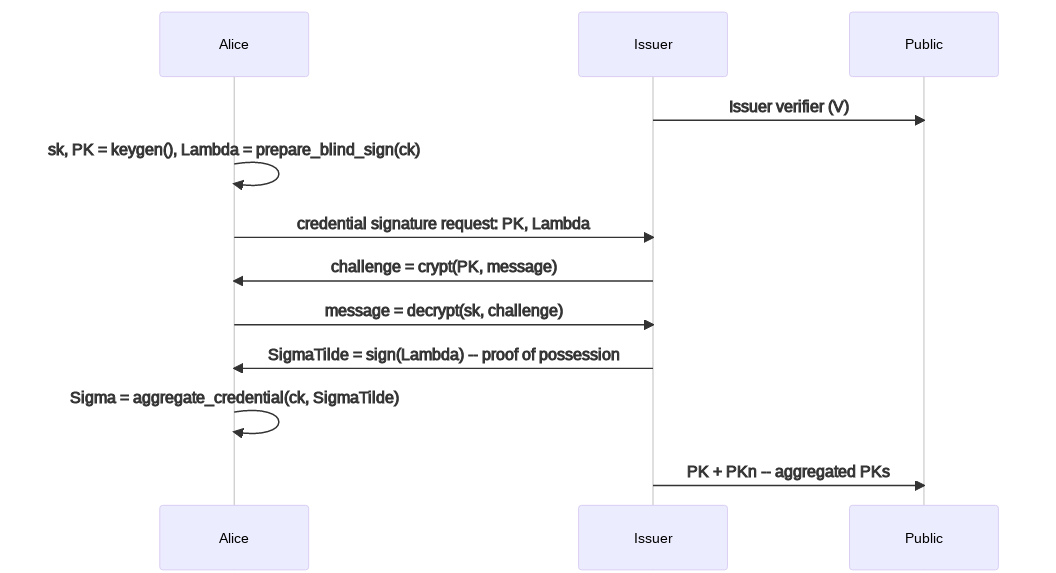
\includegraphics[width=0.4\textwidth]{keygen-seq}
\end{figure}

The following Zenroom implementation makes use of the Coconut
built-in extension for zero-knowledge proof credentials.

\begin{lstlisting}[basicstyle=\tiny,style=lua]
ZK = require_once('crypto_abc')
issuer = ZK.issuer_keygen() -- setup
sk = INT.random() -- signing key
ck = INT.random() -- credential key
PK = G2 * sk     -- signature verifier
Lambda =
 ZK.prepare_blind_sign(ck * G1, ck)
SigmaTilde =
 ZK.blind_sign(issuer.sign, Lambda)
Sigma =
 ZK.aggregate_creds(ck, {SigmaTilde})
\end{lstlisting}

This code is executed in multiple steps by the Zencode utterances:

\begin{enumerate}

\item \textbf{When I create the credential keypair}

  will create a new \emph{credential keypair} object containing
  members \emph{public} (ECP) and \emph{private} (BIG).

\item \textbf{When I create the credential request}

  will use the \emph{credential keypair} to create a new
  \emph{credential request} complex schema object for ZK proof.

\item \textbf{When I create the credential signature}

  will be executed by the Issuer after the proof-of-possession
  challenge is positive (exchange and confirmation of an encrypted
  message using BLS public keys) to sign the credential.

\item \textbf{When I create the credentials}

  will aggregate one or more \emph{credential signature} (SigmaTilde)
  together with the \emph{private} member of the \emph{credential
    keypair} and finally create \emph{credentials} capable of
  producing Zero-Knowledge proofs of possession.

\end{enumerate}



\textbf{Sign:}

\begin{figure}
  \caption{Signing process sequence diagram}
  \centering
  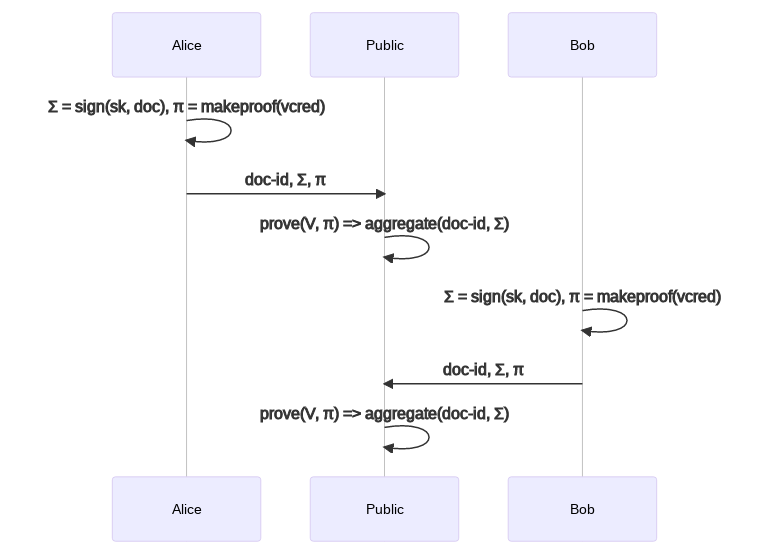
\includegraphics[width=0.4\textwidth]{sign-seq}
\end{figure}

\textbf{Verify:}

\begin{figure}
  \caption{Verification process sequence diagram}
  \centering
  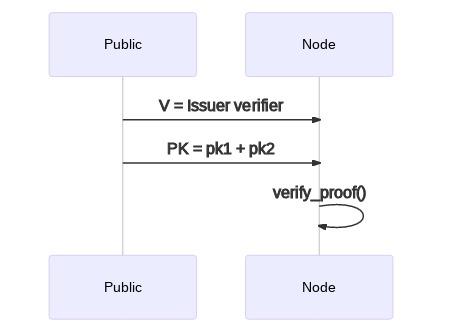
\includegraphics[width=0.4\textwidth]{verify-seq}
\end{figure}



\begin{lstlisting}[style=lua]

---------
-- SETUP
---------

G1 = ECP.generator()
G2 = ECP2.generator()

-- credentials
ZK = require_once('crypto_abc')
issuer = ZK.issuer_keygen()

-- keygen
sk1 = INT.random() -- signing key
ck1 = INT.random() -- credential key
PK1 = G2 * sk1     -- signature verifier

sk2 = INT.random()
ck2 = INT.random()
PK2 = G2 * sk2

-- issuer sign ZK credentials
Lambda1 = ZK.prepare_blind_sign(ck1*G1, ck1) -- credential request:       p -> i
SigmaTilde1 = ZK.blind_sign(issuer.sign, Lambda1)    -- issuer signs credential:  i -> p
Sigma1 = ZK.aggregate_creds(ck1, {SigmaTilde1})  -- credential sigma          p -> store

Lambda2 = ZK.prepare_blind_sign(ck2*G1, ck2)
SigmaTilde2 = ZK.blind_sign(issuer.sign, Lambda2)
Sigma2 = ZK.aggregate_creds(ck2, {SigmaTilde2})

-- sign

UID = ECP.hashtopoint(msg) -- the message's hash is the unique identifier

--------------
-- SETUP done
--------------

print "--------------------------"
print "first base signing session"
r = INT.random()
R = UID * r      -- session

-- add public keys to public session key
PM = (G2 * r) + PK1 + PK2

-- Session opener broadcasts:
-- 1. R   - base G1 point for signature session
-- 2. PM  - base G2 point for public multi-signature key
-- 3. msg - the message to be signed

-- proofs of valid signature
-- uses public session key as UID
Proof1,z1 = ZK.prove_cred_uid(issuer.verify, Sigma1, ck1, UID)
Proof2,z2 = ZK.prove_cred_uid(issuer.verify, Sigma2, ck2, UID)
-- each signer signs
S1 = UID * sk1
S2 = UID * sk2

-- generate the signature
-- each signer will communicate: UID * sk
SM = R + S1 + S2


-- print signature contents to screen
I.print({pub = PM, -- session public keys
		 sign = SM,
		 uid = UID,
		 proofhash1 = sha256( ZEN.serialize( Proof1 ) ),
		 proofhash2 = sha256( ZEN.serialize( Proof2 ) ),
		 zeta1 = z1,
		 zeta2 = z2,
		 issuer = issuer.verify
})

-- verify
assert( ZK.verify_cred_uid(issuer.verify, Proof1, z1, UID),
		"first proof verification fails")
assert( ZK.verify_cred_uid(issuer.verify, Proof2, z2, UID),
		"second proof verification fails")
assert( ECP2.miller(PM, UID)
		   == ECP2.miller(G2, SM),
        "Signature doesn't validates")

\end{lstlisting}

\section{Evaluation}
\label{sec:evaluation}

\lipsum[5]

\bibliographystyle{unsrtnat}

\bibliography{references}



% \subsection{}
% Citations use \verb+natbib+. The documentation may be found at
% \begin{center}
% 	\url{http://mirrors.ctan.org/macros/latex/contrib/natbib/natnotes.pdf}
% \end{center}

% Here is an example usage of the two main commands (\verb+citet+ and \verb+citep+): Some people thought a thing \citep{kour2014real, hadash2018estimate} but other people thought something else \citep{kour2014fast}. Many people have speculated that if we knew exactly why \citet{kour2014fast} thought this\dots

% \subsection{Figures}
% \lipsum[10]
% See Figure \ref{fig:fig1}. Here is how you add footnotes. \footnote{Sample of the first footnote.}
% \lipsum[11]

% \begin{figure}
% 	\centering
% 	\fbox{\rule[-.5cm]{4cm}{4cm} \rule[-.5cm]{4cm}{0cm}}
% 	\caption{Sample figure caption.}
% 	\label{fig:fig1}
% \end{figure}

% \subsection{Tables}
% See awesome Table~\ref{tab:table}.

% The documentation for \verb+booktabs+ (`Publication quality tables in LaTeX') is available from:
% \begin{center}
% 	\url{https://www.ctan.org/pkg/booktabs}
% \end{center}


% \begin{table}
% 	\caption{Sample table title}
% 	\centering
% 	\begin{tabular}{lll}
% 		\toprule
% 		\multicolumn{2}{c}{Part}                   \\
% 		\cmidrule(r){1-2}
% 		Name     & Description     & Size ($\mu$m) \\
% 		\midrule
% 		Dendrite & Input terminal  & $\sim$100     \\
% 		Axon     & Output terminal & $\sim$10      \\
% 		Soma     & Cell body       & up to $10^6$  \\
% 		\bottomrule
% 	\end{tabular}
% 	\label{tab:table}
% \end{table}



\end{document}
